%Ukazka zaverecne zpravy
%Posledni zmena 02/2017, Martin Cadik

\documentclass[11pt,a4paper,oneside]{article}
\usepackage[utf8]{inputenc}
%\usepackage{a4wide}
\usepackage{amsmath}
\usepackage{mathtools}
\usepackage{url}
\usepackage{algorithm}
\usepackage[noend]{algpseudocode}
\floatname{algorithm}{Alg.} 
\DeclarePairedDelimiter\ceil{\lceil}{\rceil}
\DeclarePairedDelimiter\floor{\lfloor}{\rfloor}

\usepackage{ifpdf}
\ifpdf
\usepackage[pdftex]{graphicx}
\DeclareGraphicsExtensions{.pdf,.png,.gif,.jpg}
\else
\usepackage[final]{graphicx}
\DeclareGraphicsExtensions{.eps,.png,.gif,.jpg}
\fi 

\begin{document}
	%Uvodni stranka
	\thispagestyle{empty}
	\begin{center}
	\vspace*{60mm}
	{Semestrální projekt xx -- závěrečná zpráva }\\
	\smallskip
	{\Large\bf Převod barevného obrazu na šedotónový}\\
	\smallskip
	{\it Ján Brída, \url{xbrida01@stud.fit.vutbr.cz}}\\
	\vfill
	{\bf Vedoucí práce:} {\it doc. Ing. Martin Čadík, Ph.D., \url{cadik@fit.vutbr.cz}} 
	\hfill {Květen 2017}

	\end{center}
	\newpage

	%Vlastni zprava
	\section{Úvod}
	Tento semestrální projekt se zaobírá problematikou transformace barevného obrazu
	na šedotónový. Černo-bílé fotografie se stále běžně objevují v~mnohých
	sférách vizuální prezentace, avšak~problémem šedotónové konverze bývá zachování
	detailů, především v~izoluminantních oblastech. To znehodnocuje celkový
	dojem a~sňižuje schopnost pochopit obsah obrazu.

	Bylo navrženo množství metod, kterými jsou barevné obrazy převáděny do šedotónové podoby.
	Typicky jsou rozděleny na globální a~lokální, podle toho, zda-li jsou zkoumány závislosti
	v~obraze. Prvně jmenované bývají často dostatečně rychlé, neposkytují však vždy vizuálne
	věrohodnou reprezentaci vzhledem ke vstupu. Lokální techniky se typicky snaží brát v~úvahu
	barevné změny v~oblastech a~uspůsobit podle nich výpočet luminance. Některé takovéto
	algoritmy pracují v~gradientní doméně.

	Takovýmto algoritmem je i~transformace podle experimentů s~barevným systémem
	zvaným Coloroid~\cite{cadik07color_to_gray}. Podobá se metodě~\cite{gooch2005color2gray},
	která iterativně minimalizuje chybu objektivní funkce, podle lokálních kontrastů mezi pixely, na základě
	transformace do CIE L*a*b*. Ta se snaží zachovat detaily použitím rozdílů luminance
	nebo chrominance (maximum) mezi pixely, dochází ale naneštěstí k~nekonzistencím.
	Navíc není algoritmus automaticky adaptabilní, protože vyžaduje nastavení
	trojice parametrů ovlivňující výslednou transformaci.

	\section{Šedotónová transformace}
	Jedná se o~redukci alespoň 3 barevných složek (např. RGB) na 1D data.
	Jak bylo zmíněno, výzvou takovéhoto převodu je zachovat ekvivalentní
	přechody v~novém obraze, aby byl výsledek percepčně blízký vstupu.

	\subsection{Coloroid}
	Barevný systém Coloroid byl vytvořen pro popsání spojitého barevného prostoru,
	který je esteticky uniformní protože dokáže definovat harmonické vztahy mezi barvami,
	jelikož sousedící barvy jsou určeny stejně velkými celočíselnými intervaly.
	Spojitost barevného prostoru Coloroidu poskytuje možnost jednoznačne určit
	vztahy mezi barvami v~jiných barevných systémech. Coloroid vynalezli v~60.-80. letech
	minulého staletí v~Budapešti na základě experimentů při sledování barev pozorovatelem,
	celkově bylo těchto jednotlivců až $70\,000$.

	Barvy jsou v~tomto 3D prostoru definovány pomocí HSL (\emph{hue}, \emph{saturation},
	\emph{luminance}) komponent (obrázek~\ref{fig:coloroid}).
	Coloroid reprezentuje válec, kde angulární souřadnice
	(A) určuje odstín, nasycení definuje radiální souřadnice (T) a~na vertikální ose (V)
	se pohybuje svítivost barvy. Důležitou informací je, že s~nulovou saturací je barva
	reprezentována v~šedotónové oblasti. 48 základních barev  v~základni kužele
	představuje vztah k~CIE 1931 barevnému gamutua~nejvíce nasycené mají hodnoty na obvodu tohoto kruhu.

	V~práci~\cite{cadik07color_to_gray} je Coloroid využit pro převod na percepčně blízký šedotónový výsledek
	vstupního obrazu. Autoři provedli sledování několika barev, kde náhle jedna z~nich byla
	nahrazena za nesaturovaný vzorek. Pozorovatel po změně zhodnotil uniformitu vnímání v~krátkém
	čase (aby oko nemělo čas se přispůsobit). Na základě těchto experimentů došlo na
	substituci šedotónových vzorků do vygenerovaných posloupností s~fixními A, V komponentami
	a~postupně rostoucí saturací. Výsledkem byl poznatek, že nedochází k~monotónní diferenci mezi
	těmito vzorky v~šedotónové oblasti.

	Byla vytvořena matice $7 \times 7$ šedotónových změn mezi 7 vybranými odstíny (zástupci 7 skupin
	základních barev Coloroidu). Na diagonále se vyskytují nuly a~je anti-symetrická, viz
	jak byly hodnoty naměřeny~\cite{cadik07color_to_gray}. Tato matice je základním stavebním prvkem pro převodovou
	rovnici na šedotónovou podobu. Zbylé barvy získají své diference bilineární interpolací.

	\begin{figure}[htb]
		\centering
		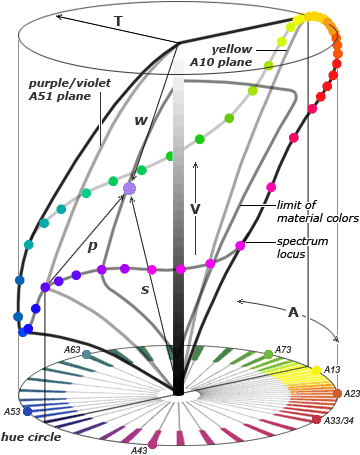
\includegraphics[scale=0.5]{fig/Coloroid.png}
		\caption{Model barevného prostoru Coloroid.} 
		\label{fig:coloroid}
	\end{figure}

	\subsection{Rovnice pro šedotónovou transformaci}
	Hledanou veličinou je gradient, popisující rozdíl mezi dvěmi Coloroid
	barvami $(A_1, T_1, V_1)$, $(A_2, T_2, V_2)$ a~je vypočten podle
	rovnice~\eqref{eq:grad}. Ta obsahuje termy diferencí luminance
	(rovnice~\eqref{eq:lum}), saturace (rovnice~\eqref{eq:sat}) a~odstínu
	(rovnice~\eqref{eq:hue}), postupně odvozeny na základě~tabulky změn
	pro 7 barevných skupin.

	\begin{equation}
		\Delta_{1, 2} = dL(L_1, L_2) + S(A_1, T_1, V_1, A_2, T_2, V_2) + h(A_1, T_1, A_2, T_2)
		\label{eq:grad}
	\end{equation}

	Gradient odstínu dvou barev $A_1$, $A_2$ je vypočten jako
	\begin{equation}
		h(A_1, T_1, A_2, T_2) = w_h \cdot H(A_1, A_2) \cdot \sqrt{u(T_{1rel}) \cdot u(T_{2rel})},
		\label{eq:hue}
	\end{equation}
	kde $T_{rel}$ je relativní saturace pro každou rovinu odstínů v~každé úrovni luminance.
	Term $u(x)$, kde $x = 2 \cdot T_{rel}$, je definován jako $u(x) = 0.5 \cdot x$, pokud $x < 0.5$
	a~$u(x) = \sqrt{x} - 0.5$ jinak.

	Určení šedotónové změny pro korespondující saturaci závisí na
	\begin{equation}
		S(A_1, T_1, V_1, A_2, T_2, V_2) = w_s \cdot \left[S(A_2, T_2, V_2) - S(A_1, T_1, V_1)\right]
		\label{eq:sat}
	\end{equation}
	a~pro luminanci
	\begin{equation}
		dL(L_1, L_2) = L_2 - L_1,
		\label{eq:lum}
	\end{equation}
	jak je podrobněji rozebráno odvození těchto rovnic v~\cite{cadik07color_to_gray}.

	\subsection{Výpočet na základě gradientního pole}
	Obdržený nekonzistentní gradientní obraz je následně stabilizován pomocí speciální metody, užívající
	ortogonální projekci pro nalezení nejbližšího konzistentního gradientního pole. Výsledek
	tohoto procesu je nakonec zpracován integrací podle navštíveného gradientu~\cite{cadik07color_to_gray}.

	Hlavní myšlenkou korekce gradientního pole $\mathbf{g}$ je určit chybu $E_{(i, j)}$
	jednotlivých elementárních smyček všech pixelů. Konzistentní gradientní pole po
	této úpravě musí splňovat rovnost
	$$
		\mathbf{g}_{(i + 1, j), x} + \mathbf{g}_{(i, j), y} =
		\mathbf{g}_{(i, j), x} + \mathbf{g}_{(i, j + i), y}.
	$$

	Algoritmus opakovaně prochází daný obraz a~pro každý pixel spočte $E_{(i, j)}$ podle výše uvedeného
	vztahu. Chyba je pak distribuována, čímž je obdržen nový gradient $\mathbf{g}(i, j)$. Definice
	numerické metody představuje
	\begin{equation}
		\mathbf{g}^{(k + 1)} = \mathbf{g}^{(k)} - \frac{1}{4} \cdot E_{(i, j)} \cdot \mathbf{N}_{(i, j)},
	\end{equation}
	kde $\mathbf{N}_{(i, j)} = (0, \dots, 0, +1, +1, -1, -1, 0, \dots, 0)$ identifikuje $2 \cdot
	N \cdot M$ vektor s~odpovídajícími nenulovými koeficienty pro $\mathbf{g}_{(i,j)}$, kde $N$
	je výška a~$M$ šířka obrazu. $E_{(i, j)}$ postupně konverguje k~nule. V~algoritmu~\ref{alg:correct_grad}
	představuje $1 < \omega < 2$ urychlení konvergence.

	\begin{algorithm}
		\caption{Sekvenční algoritmus korekce gradientního pole $\mathbf{g}$.}
		\label{alg:correct_grad}
		\begin{algorithmic}[1]
			\Function{correct gradient}{$\mathbf{g}$, $\omega$, $\epsilon$}
				\Repeat
					\State $E_{\max} \gets 0$
					\For{$i \in \left\{0, \dots, N\right\}$}
						\For{$j \in \left\{0, \dots, M\right\}$}
							\State $E \gets \mathbf{g}_{(i + 1, j),x } + \mathbf{g}_{(i, j), y} -
									\mathbf{g}_{(i, j), x} - \mathbf{g}_{(i, j + i), y}$

							\If{$|E| > E_{\max}$}
								\State $E_{\max} \gets |E|$
							\EndIf
							
							\State $E \gets \frac{1}{4} \cdot E \cdot \omega$

							\State $\mathbf{g}_{(i, j), x} \gets \mathbf{g}_{(i, j), x} - E$
							\State $\mathbf{g}_{(i, j + 1), y} \gets \mathbf{g}_{(i, j + 1), y} - E$
							\State $\mathbf{g}_{(i + 1, j), x} \gets \mathbf{g}_{(i + 1, j), x} + E$
							\State $\mathbf{g}_{(i, j), y} \gets \mathbf{g}_{(i, j), y} + E$
						\EndFor
					\EndFor
				\Until{$E_{\max} > \epsilon$}
			\EndFunction
		\end{algorithmic}
	\end{algorithm}

	\subsubsection{Optimalizace}
	Výše uvedený algoritmus je cyklickým řešením korekce gradientu jeho elementárních smyček obrazu.
	Urychlení výpočtu pomocí data paralelních algoritmů na grafické kartě rozděluje algoritmus
	na 3~zájmová místa (následující výčet referuje řádky algoritmu~\ref{alg:correct_grad}):
	\begin{enumerate}
		\item \#6: paralelní výpočet chyby $\mathbf{E}_{(i, j)}$ všech elementárních smyček,
		      kde $\mathbf{E}$ je vektor o~velikosti $N \cdot M$,
		\item \#7-8: redukce $\mathbf{E}$ s~asociativním operátorem $\max$ pro získání $E_{\max}$,
		\item \#10-13: aby nedocházelo k~čtecím/zápisovým~datovým konfliktů, jsou jednotlivé
		      přiřazení výsledků provedeny paralelně samostatně.
	\end{enumerate}

	Je možné vytvořit i~efektivnejší modifikaci této korekce výběrem upravované elementární smyčky
	na základě maximální chyby $E_{\max}$ v~jedné iteraci algoritmu~\cite{cadik07color_to_gray}.
	Určení elementární smyčky s~$E_{\max}$ v~paralelním prostředí může být zjednodušeno na nalezení
	odpovídajícího indexu pixelu během redukce $\mathbf{E}$. Index je jednoduše definován pracovním
	identifikátorem výpočtu a~dodatečne vyžaduje $\ceil*{N \cdot M}_{(2 \cdot W)} \div {(2 \cdot W)}$
	paměťového místa pro uchování této informace při rekurzivní redukci, kde $W$ určuje velikost
	pracovní skupiny.

	\begin{figure}[htb]
		\centering
		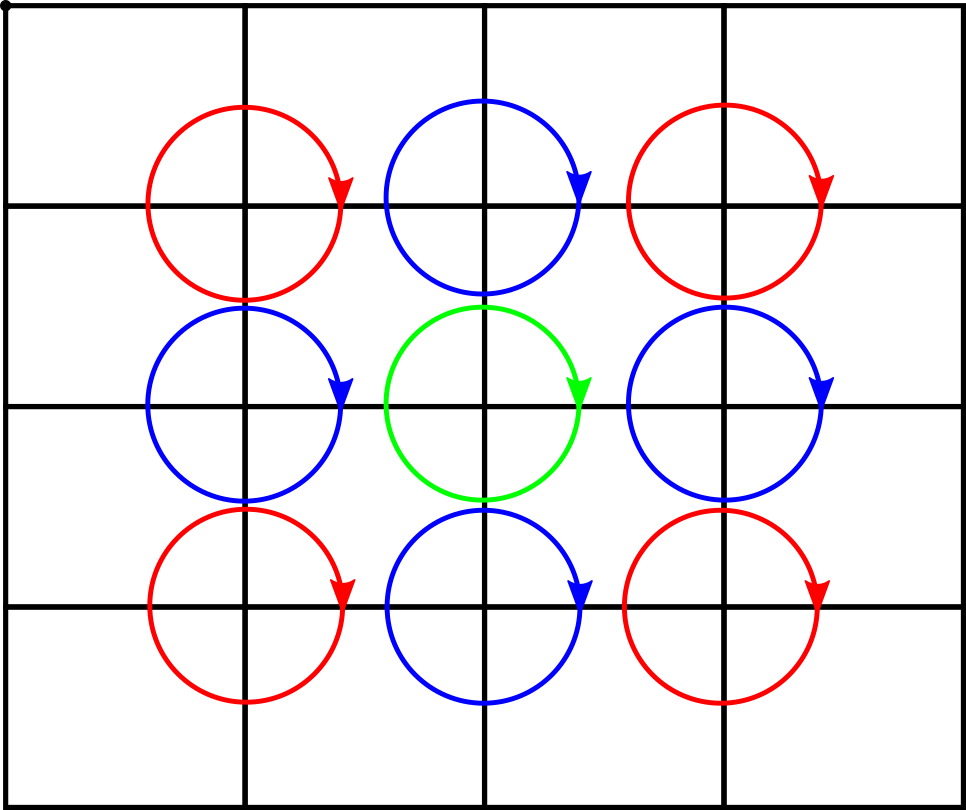
\includegraphics[scale=0.3]{fig/chess.png}
		\caption{Šachovnicovitá korekce gradientu. Pouze smyčky jedné barvy jsou prováděny paralelně.}
		\label{fig:chess}
	\end{figure}

	Další optimalizační návrh představuje \emph{šachovnicový} průchod gradientním polem. Tento způsob
	korekce gradientu je vyobrazen na obrázku~\ref{fig:chess}. Metoda je rozdělena do 3 volání kernelu
	pro výpočet chyby elementárních smyček. V~jednotlivých voláních jsou aktualizovány pouze jisté smyčky,
	aby nedocházelo ke zapisovacím konfliktům. To znamená, pro $[i, j]$, kdy:
	\begin{itemize}
		\item $i \bmod 2 = 0 \wedge j \bmod 2 = 0$,
		\item $(i \bmod 2 \neq 0 \wedge j \bmod 2 = 0) \lor (i \bmod 2 = 0 \wedge j \bmod 2 \neq 0)$,
		\item $i \bmod 2 \neq 0 \wedge j \bmod 2 \neq 0$.
	\end{itemize}
	Tento typ modifikování gradientního pole má dobré předpoklady paralelně distribuovat chybu
	a~tím jakkoby rozmazávat lokální nekonzistence.

	Poslední z~navržených řešení staví na hierarchickém rozdělení gradientního pole obrazu do
	stromové struktury quadtree. Úmyslem je snadněji identifikovat oblasti, ve kterých je
	chyba elementárních smyček je nad prahem $\epsilon$ a~pouze tyto smyčky opravovat. Pro jednoduché paralelní
	vybudování quadtree se gradientní pole uloží podle $z$-křivky do 1D pole. Uzly ve vyšší
	úrovni quadtree sumují hodnoty svých potomků a~podle uspořádání v~$z$-křivce platí:
	\begin{equation}	
		Q_{(i)}^n = Q_{(4 \cdot i)}^{n - 1} + Q_{(4 \cdot i + 1)}^{n - 1} +
		            Q_{(4 \cdot i + 2)}^{n - 1} + Q_{(4 \cdot i + 3)}^{n - 1}
		\label{eq:avg}
	\end{equation}
	Takto obydlený quadtree už lze použít pro hierarchickou korekci, třeba si však uvědomit,
	že v~každé iteraci budou muset být znovu vypočteny vyšší úrovně. Následující body popisují
	průběh algoritmu:
	\begin{enumerate}
		\item přepočti vyšší úrovně quadtree,
		\item inicializuj seznam $\textsc{ParentIndex}_{n - 2}$ na indexy~všech uzlů $n - 2$ úrovně (je jich spolu 16),
		      nastav počet zpracovávaných uzlů na $N_i^a = 64$
		\item postupuj sestupně v~quadtree od úrovně $n - 3$, pro každou úroveň proveď:
		\begin{enumerate}
			\item vypočti chybu $E$ v~úrovni $i$ pro potomky uzlů indexovaných podle $\textsc{ParentIndex}_{i + 1}$,
			      zároveň ulož Mortonový kódy těchto potomků do seznamu $\textsc{ActNodes}_i$ a~inicializuj
			      nový seznam $\textsc{Flag}_i$ tak, aby se pro smyčky, kterých hodnota $|E| > \epsilon$, byla
			      uložena na odpovídajícím indexu $1$, jinak $0$,
			\item proveď exkluzivní sken nad $\textsc{Flag}_i$, výsledek ulož do seznamu $\textsc{Offsets}_i$,
			\item $N_{i - 1}^a = \textsc{Flag}_{i, (N_i^a - 1)} + \textsc{Offsets}_{i, (N_i^a - 1)}$,
			\item pokud $N_i^a = 0$ skonči průchod stromem,
			\item uskutečni kompakci $\textsc{ActNodes}_i$ podle $\textsc{Flag}_i$ na pozici definované $\textsc{Offsets}_i$,
			      výsledkem bude $\textsc{ParentIndex}_i$ o~velikosti $N_{i - 1}^a$,
			\item $N_{i - 1}^a = 4 \cdot N_{i - 1}^a$.
		\end{enumerate}
		\item pokud $N_0^a = 0$ skonči iterativní algoritmus,
		\item proveď šachovnicovou korekci gradientu podle $\textsc{ParentIndex}_1$,
		      chyba se zapisuje do seznamu $\textsc{Error}_0$,
		\item redukuj $\textsc{Error}_0$ pro nalezení absolutního maxima $E_{\max}$,
		\item pokud $E_{\max} > \epsilon$ vrať se na krok \#1, jinak skonči.
	\end{enumerate}

	\section{Implementace}
	Implementace v~jazyce C++ používá zdrojový kód od Laszla Neumanna pro výpočet gradientu luminance
	podle Coloroidu. Optimalizace korekce gradientu proběhla za pomoci GPGPU OpenCL API. Toto rozhraní
	je zapouzdřeno do vlastních tříd v~jmenném prostoru \texttt{cl} (složka \texttt{compute}). Program
	samostatně implementuje redukci i~exkluzivní sken. Program byl napsán jako plugin do aplikace
	\texttt{TMOcmd}/\texttt{TMOgui}, proto hlavní třídu přestavuje \texttt{TMOCadik08},
	která se stará nejen o~vstupní parametry, ale ovládá i~celkový průběh konverze.

	Nejdpostatnější část korekce gradientu sa nachází v~metodě \\
	\texttt{TMOCadik08::correctGrad}. Ta volá kernely definované \\
	v~\texttt{resources/kernels/color2gray.cl} a~řídí proces iterativní
	korekce gradientu. Implementováno bylo několik verzí, jak bylo naznačeno v~předcházející kapitole.

	\textbf{Cyklická korekce gradientu:} \; naivní implementace algoritmu prakticky opisuje
	paralelní variantu algoritmu~\ref{alg:correct_grad}. Nejprve jsou do vektoru $\textbf{E}$
	vypočteny chyby všech elementárních smyček. Poté sa provede korekce a~také redukce $\textbf{E}$
	pro nalezení maximální chyby $E_{\max}$.

	\textbf{Korekce maximální chyby:} \; tato varianta poskytuje výpočet $\textbf{E}$ a~nalezení
	$E_{\max}$ podobně jako v~předcházející verzi, korekce se však provádí jen pro smyčku s~$E_{\max}$.
	Nalezení indexu elementární smyčky s~odpovídající maximální chybou lze provést během redukce.
	Dodatečně se použijí seznamy odpovídajících indexů parciálních zpracování vstupního pole.

	\textbf{Šachovnicová korekce gradientu:} \; tato verze vychází z~principu vyobrazeném
	v~obrázku~\ref{fig:chess}. Podobně jako dříve sa vypočte $\textbf{E}$ a~pomocí redukce absolutního maxima
	je nalezeno $E_{\max}$. Korekce probíhá ve 3 cyklech, kdy proměnná \texttt{mode} identifikuje aktuálně
	zpracovávané elementární smyčky.

	\textbf{Hierarchická korekce gradientu pomocí $z$-uspořádaného quadtree:} \;
	soubory \texttt{morton.h} a~\texttt{morton.cpp} definují kódování/dekódování Mortonových kódů.
	Pro urychlení těchto procesů jsou předpočítány byty Mortonových kódů do shiftovacích look-up
	tabulek. Třída \texttt{quadtree} (\texttt{quadtree.h} \\ a~\texttt{quadtree.cpp})
	zřejmě poskytuje zapouzdření quadtree pro obrazový gradient. Alokace probíhá podobně jako pro 4-ární
	strom, ovšem v~každé úrovni jsou uzly uspořádány podle $z$-křivky. Korekce gradientu
	probíhá zase iterativně při selekci maximální chyby $E_{\max}$ z~$\textbf{E}$, ovšem
	$\textbf{E}$ je redukované gradientní pole na základě průchodu stromem. Přepočtení vyšších
	úrovní v~quadtree se děje v~kernelu \texttt{avg\_grad} podle vzorce~\eqref{eq:avg}.
	Kernel \texttt{calc\_error} provádí selekci potomků na zpracování v~další úrovni
	nastavením bufferu $\textsc{Flag}_i$. $\textsc{ActNodes}_i$ jsou vypočítány jako
	$ (\textsc{ParentIndex}_{i + 1, (j)} / 4] \ll 2) \mid (j \bmod 4)$, kde $j$ je číslo
	pracovního objektu. Exkluzivním skenem jsou zjištěny ofsety a~kompakcí se určí následující
	Mortonovy kódy aktivních uzlu ($\textsc{ParentIndex}_i$). Nakonec se korekce gradientu provede
	podobně jako v~předchozí variantě.

	\textbf{Další:} \; za zmínku stojí pokus o~korekci gradientu s~procházením delší cesty.
	Vyskoušena byla \emph{spirálovitá} varianta, kdy smyčky postupně snižují svoji velikost
	jak se blíží ke středu obrazu. Problémem takovéhoto průchodu bylo nerovnoměrné zatížení vláken.
	Uvažována byla i~varianta Hilbertovy křivky, tzv. Moorova křivka, které počátek a~konec
	představují sousední uzly (je tedy prakticky uzavřená), ovšem nebyly k~dispozici gradienty
	do všech směrů (jejich výpočet podle dostupných kódu způsobil \emph{segmentation fault}).

	Také byla implementována paralelní verze integrace výsledného gradientního pole. Integrace
	probíhá nejprve sekvenčně pro první sloupec obrazu ve směru osy Y, následně se pro
	každý řádek provede výpočet na základě komponenty $x$. Nad výsledným obrazem
	se nakonec provede kalibrace.

	\section{Výsledky}
	Testování proběhlo nad sérií obrázků z~\url{http://cadik.posvete.cz/color_to_gray_evaluation}.
	Mnoho z~nich poskytuje dobré případy izoluminantních oblastí, ktéré by se v~klasické konverzy
	podle CIE Y vytratily. Pro studium estetických rozdílů byl zvolen obrázek~\ref{fig:in}.
	Z~důvodu nefunkčních ovladačů OpenCL na GNU/Linux a~problému při překladu \texttt{TMS}
	na Windows bylo naneštěstí prozatím volání kernelů vykonáno na CPU.

	\begin{figure}[!htbp]
		\centering
		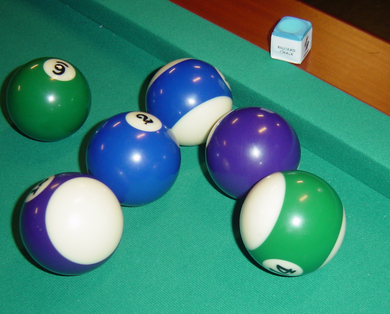
\includegraphics[scale=0.5]{../resources/images/balls.jpg}
		\caption{Testovaný obrázek.}
		\label{fig:in}
	\end{figure}

	Výsledky: \\
	\textbf{Cyklická korekce gradientu:} \;
	$\epsilon = 0.5$, 0.273868 [s]. \\
	\textbf{Korekce maximální chyby:} \;
	$\epsilon = 0.5$, více jak 5 [s]. \\
	\textbf{Šachovnicová korekce gradientu:} \;
	$\epsilon = 1.5$, 0.0630407 [s]. \\
	\textbf{Hierarchická korekce gradientu:} \;
	$\epsilon = 0.1$, 0.464364 [s]. \\

	\begin{figure}[!htbp]
		\centering
		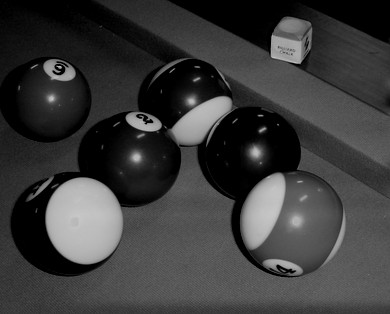
\includegraphics[scale=0.4]{fig/balls_cyc.jpg}
		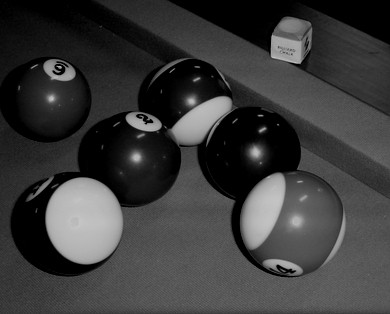
\includegraphics[scale=0.4]{fig/balls_mer.jpg}
		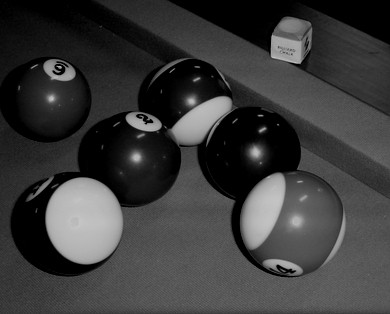
\includegraphics[scale=0.4]{fig/balls_chess.jpg}
		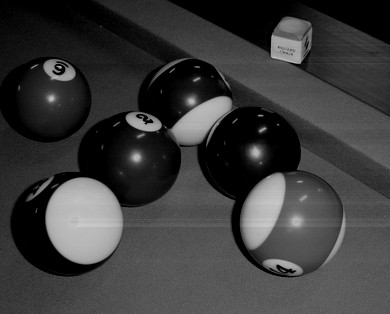
\includegraphics[scale=0.4]{fig/balls_hier.jpg}
		\caption{Výsledek konverze: cyklické, max.,
		         šachovnicové, hierarchické.}
		\label{fig:res_cyc}
	\end{figure}

	\subsection{Uživatelská studie}
	Z~výsledků výše je patrné, které varianty jsou nejpoužitelnejší.
	Nejlépe si vedla korekce podle šachovnicového vzoru. Ta dokáže i~při poměrně
	vysokém $\epsilon$ distribuovat chybu tak, aby byl výsledek stále přijatelný
	a~tím také omezí délku trvání algoritmu. Naivní cyklická korekce bohužel
	neposkytuje dostatečné zrychlení a~navíc způsobuje dodatečné artefakty. 
	Korekce maximální chyby nepřineslo slibované zrychlení, i~když metoda dokáže
	poměrně účinně odstranit nekonzistence. U~hierarchické korekce se momentálně
	zdá být problematické používat ve vyšších úrovních průměrnou hodnotu gradientu
	potomků. Pravděpodobně bude nutné upravit porovnávání s~$\epsilon$ anebo změnit typ informace,
	která bude uložena.

	\section{Závěr}
	...

	\bibliographystyle{acm}
	\bibliography{report}
\end{document}
